\chapter{Diseño e Implementación} % Main chapter title

\label{Chapter3} % Change X to a consecutive number; for referencing this chapter elsewhere, use \ref{ChapterX}

\definecolor{mygreen}{rgb}{0,0.6,0}
\definecolor{mygray}{rgb}{0.5,0.5,0.5}
\definecolor{mymauve}{rgb}{0.58,0,0.82}

%%%%%%%%%%%%%%%%%%%%%%%%%%%%%%%%%%%%%%%%%%%%%%%%%%%%%%%%%%%%%%%%%%%%%%%%%%%%%
% parámetros para configurar el formato del código en los entornos lstlisting
%%%%%%%%%%%%%%%%%%%%%%%%%%%%%%%%%%%%%%%%%%%%%%%%%%%%%%%%%%%%%%%%%%%%%%%%%%%%%
\lstset{ %
  backgroundcolor=\color{white},   % choose the background color; you must add \usepackage{color} or \usepackage{xcolor}
  basicstyle=\footnotesize,        % the size of the fonts that are used for the code
  breakatwhitespace=false,         % sets if automatic breaks should only happen at whitespace
  breaklines=true,                 % sets automatic line breaking
  captionpos=b,                    % sets the caption-position to bottom
  commentstyle=\color{mygreen},    % comment style
  deletekeywords={...},            % if you want to delete keywords from the given language
  %escapeinside={\%*}{*)},          % if you want to add LaTeX within your code
  %extendedchars=true,              % lets you use non-ASCII characters; for 8-bits encodings only, does not work with UTF-8
  %frame=single,	                % adds a frame around the code
  keepspaces=true,                 % keeps spaces in text, useful for keeping indentation of code (possibly needs columns=flexible)
  keywordstyle=\color{blue},       % keyword style
  language=[ANSI]C,                % the language of the code
  %otherkeywords={*,...},           % if you want to add more keywords to the set
  numbers=left,                    % where to put the line-numbers; possible values are (none, left, right)
  numbersep=5pt,                   % how far the line-numbers are from the code
  numberstyle=\tiny\color{mygray}, % the style that is used for the line-numbers
  rulecolor=\color{black},         % if not set, the frame-color may be changed on line-breaks within not-black text (e.g. comments (green here))
  showspaces=false,                % show spaces everywhere adding particular underscores; it overrides 'showstringspaces'
  showstringspaces=false,          % underline spaces within strings only
  showtabs=false,                  % show tabs within strings adding particular underscores
  stepnumber=1,                    % the step between two line-numbers. If it's 1, each line will be numbered
  stringstyle=\color{mymauve},     % string literal style
  tabsize=2,	                   % sets default tabsize to 2 spaces
  title=\lstname,                  % show the filename of files included with \lstinputlisting; also try caption instead of title
  morecomment=[s]{/*}{*/}
}


%----------------------------------------------------------------------------------------
%	SECTION 1
%----------------------------------------------------------------------------------------
%\section{Análisis del software}
% 
%La idea de esta sección es resaltar los problemas encontrados, los criterios utilizados y la justificación de las decisiones que se hayan tomado.
%
%Se puede agregar código o pseudocódigo dentro de un entorno lstlisting con el siguiente código:
%
%\begin{verbatim}
%\begin{lstlisting}[caption= "un epígrafe descriptivo"]
%	las líneas de código irían aquí...
%\end{lstlisting}
%\end{verbatim}
%
%A modo de ejemplo:
%
%\begin{lstlisting}[label=cod:vControl,caption=Pseudocódigo del lazo principal de control.]  % Start your code-block
%
%#define MAX_SENSOR_NUMBER 3
%#define MAX_ALARM_NUMBER  6
%#define MAX_ACTUATOR_NUMBER 6
%
%uint32_t sensorValue[MAX_SENSOR_NUMBER];		
%FunctionalState alarmControl[MAX_ALARM_NUMBER];	//ENABLE or DISABLE
%state_t alarmState[MAX_ALARM_NUMBER];						//ON or OFF
%state_t actuatorState[MAX_ACTUATOR_NUMBER];			//ON or OFF
%
%void vControl() {
%
%	initGlobalVariables();
%	
%	period = 500 ms;
%		
%	while(1) {
%
%		ticks = xTaskGetTickCount();
%		
%		updateSensors();
%		
%		updateAlarms();
%		
%		controlActuators();
%		
%		vTaskDelayUntil(&ticks, period);
%	}
%}
%\end{lstlisting}

%Es este capítulo se presentarán las topologías básicas del sistema ferroviario y los dos enfoques de resolución del proyecto, con sus ventajas y desventajas antes de abordar la implementación de la solución elegida.

En este capítulo se presentarán las decisiones de diseño adoptadas para concretar el desarrollo del trabajo. Además de describir en forma genérica los módulos necesarios tanto del sistema de enclavamiento como de los bloques auxiliares para concretar una comunicación exitosa entre el sistema y el exterior.

\section{Consideraciones generales}

En el presente trabajo se optó por implementar el sistema bajo el enfoque funcional. Asumiendo que sus ventajas son mucho mas fuertes que sus desventajas y el análisis de los resultados obtenidos fueron mucho mas provechosos que los de su contraparte funcional.

Los módulos del sistema fueron implementados con máquinas de estado finitas con camino de datos (FSMD, del inglés \textit{Finite State Machine with Data path}), que son máquinas de estado finitas (FSM, del inglés \textit{Finite State Machine}) y circuitos secuenciales. La FSMD (Figura \ref{fig:FSMD}) posee dos partes diferenciadas: el camino de control y el camino de datos. El camino de control contiene una FSM que ,según las entradas de control y el estado interno que posee, genera señales de control internas que controlan los circuitos secuenciales del camino de datos que contienen los bloques que procesan las entradas y actúan sobre las salidas.

	\begin{figure}[h]
	\centering
		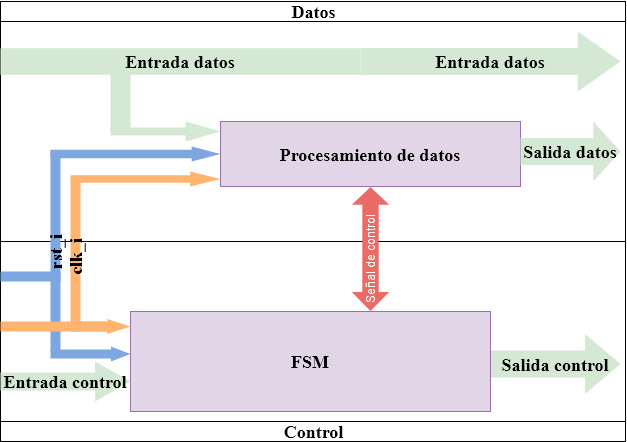
\includegraphics[scale=.5]{./Figures/FSMD}
		\caption{Diagrama en bloques genérico de una FSMD}
		\label{fig:FSMD}
	\end{figure}
	
	\vspace{5cm}
	
	Siguiendo los lineamientos recomendados, una FSMD debe ser diseñada, implementada y simulada siguiendo los siguientes pasos:
	
	\begin{enumerate}
		\item Definición del algoritmo a implementar.
		\item Definición de entradas y salidas de la FSMD.
		\item Diseño del camino de datos.
		\item Diseño de interfaz entre camino de datos y camino de control.
		\item Definición de los estados de la FSM.
		\item Diseño de la FSM.
		\item Implementar el diseño.
		\item Diseñar e implementar los ensayos.
	\end{enumerate}
	
	Esta metodología puede inferir mas tiempo de desarrollo que el habitual, pero ya ha demostrado ser exitosa en el proyecto realizado por el Mg. Ing. Facundo Larosa, codirector de este trabajo. Por lo que se aprovechó su experiencia y conocimiento para resolver esta etapa del desarrollo. Los beneficios son un mayor control del diseño a bajo nivel, una mayor portabilidad y un mas eficiente uso de los recursos de la plataforma electrónica.

\section{Plataforma utilizada}

	Por razones de disponibilidad se utilizó el kit de desarrollo Arty Z7  (Figura \ref{fig:FPGA}), el cual posee 17600 LUT’s, 35200 FF’s, 32 BUFG’s y 100 IOB’s \cite{cite28}. Se lo utilizó como base para sintetizar el diseño y extraer conclusiones que permitan dimensionar los recursos lógicos necesarios para un desarrollo de estas características.
	
	\begin{figure}[h]
	\centering
		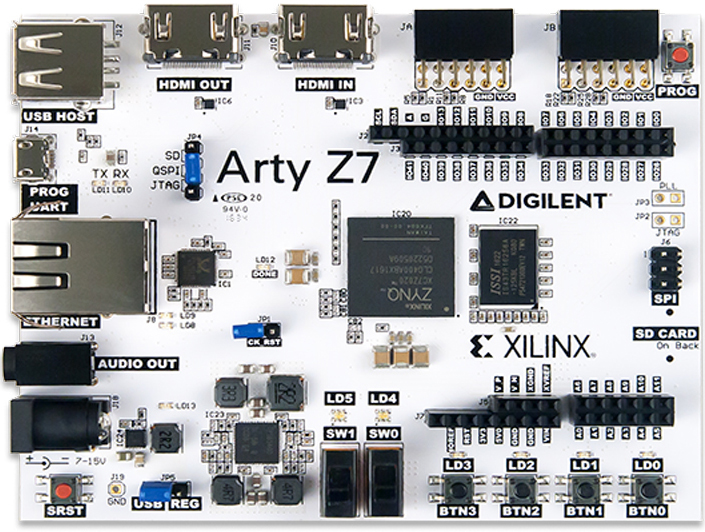
\includegraphics[scale=.4]{./Figures/FPGA}
		\caption{FPGA Arty Z7-10 de Digilent}
	\label{fig:FPGA}	
	\end{figure}

\section{Análisis de la red ferroviaria y generación automática del código}

	Todo grafo ferroviario necesita dos datos para estar definido. El primero es la una lista de relaciones entre nodo inicial y nodo final, el segundo es la posición absoluta del nodo en el grafo junto con datos adicionales como si posee un paso a nivel o si es bidireccional. Con esa información es posible realizar un análisis para obtener un resultado como el que se presenta en la Figura \ref{fig:Mapa} al ingresar un grafo de una red ferroviaria bypass.	

	\begin{figure}[h]
	\centering
		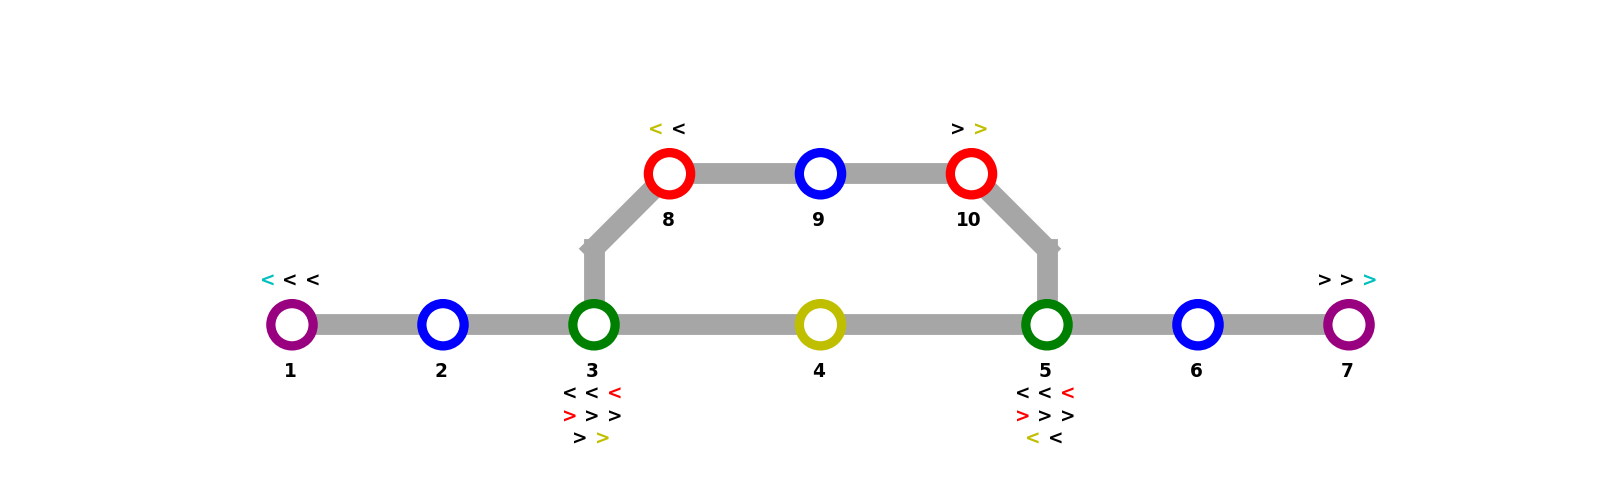
\includegraphics[scale=.4]{./Figures/Mapa_2}
		\caption{Grafo luego de ser analizado por el algoritmo}
		\label{fig:Mapa}
	\end{figure}

	Los nodos 1 y 7 se encuentran pintados de violeta porque al tener un único vecino cada uno se consideran nodos extremos. Los nodos 2,6 y 9 no presentan nada en especial por lo que son nodos simples. Los que si tienen una importancia central en el análisis son los nodos que poseen tres vecinos: el nodo 3 y el nodo 5, que son pintados en verde y se consideran cambios raíz.

	Luego el nodo 4 es categoriza como nodo cambio directo por ser la continuación de los segmentos 2-3 y 5-6 de tener el cambio de vía en posición normal, permitiendo la circulación directa. En este caso el nodo 4 es compartido por ambos cambios pero no siempre se da este caso.
	
	Los nodos 8 y 10, siendo vecinos de los cambios 3 y 5 pero no compartiendo ninguna coordenada espacial con ellos, son nodos de cambios ramificados. Es decir, solo permitirán la secuencia de nodos 2-3-8 o 9-8-3 si la máquina de cambios se encuentra en posición inversa. Para el nodo 5 el análisis es análogo.

	La asignación de semáforos se realiza solo sobre los nodos extremos, cambios raíz y cambios ramificados. Los extremos necesitan los semáforos para permitir la salida de las formaciones de la red, ya que la red ferroviaria continua mas allá del nodo 1 y del 7, de ser nodos extremos absolutos (fin de red) no corresponde que se les asigne un semáforo.
	
	Los nodos de cambios son los que presentan mayor cantidad de semáforos. Necesitan dos semáforos de tres aspectos para permitir la circulación directa sobre el cambio cuando se encuentra en posición normal y un semáforo de dos aspectos para permitir la circulación en la ramificación del recorrido, pero con precaución por ser una zona crítica. Finalmente los nodos de cambios ramificados solo presentan un semáforo de doble aspectos como complemento al otro semáforo de maniobras, para permitir utilizar la ramificación para volver al recorrido principal a una velocidad moderada. 

\section{Módulo de nodos}

	Como existen diversos tipos de nodos instanciados en el sistema, se describirá el funcionamiento de un nodo genérico con la máxima cantidad de funcionalidades, de forma tal de cubrir todos los casos.
	
	Un módulo de nodo (cuyo diagrama de bloques se presenta en la Figura \ref{fig:FSMD_Nodo}) recibe los estados de ocupación de sus vecinos y de si mismo desde el exterior, además del estado de los semáforos que posee. 
	
	\begin{figure}[h]
	\centering
	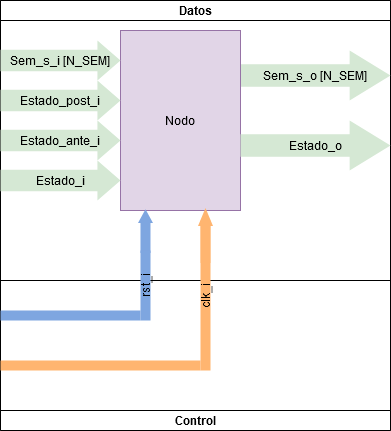
\includegraphics[scale=.5]{./Figures/FSMD-Nodo}
		\caption{FSMD del módulo de nodo genérico}
		\label{fig:FSMD_Nodo}
	\end{figure}		
	
	Internamente deberá informar su estado de ocupación a sus vecinos y decidir los aspectos que deberán tener sus semáforos de la siguiente manera:
			
	\begin{itemize}
		\item Si el tramo propio está ocupado: el semáforo propio estará en aspecto rojo.
		\item Si el vecino está ocupado: el semáforo propio estará en aspecto rojo.
		\item Si el vecino está desocupado:
		\begin{itemize}
			\item Si el semáforo vecino está en rojo: el semáforo analizado estará en aspecto amarillo.
			\item Si el semáforo vecino está en amarillo:  el semáforo analizado estará en aspecto verde.
		\end{itemize}				 
	\end{itemize}
	
\section{Módulo de la máquina de cambios cambios}

	Un cambio de vías en la realidad conecta un tramo A con un tramo B o con un tramo C. Pero en la implementación de los nodos solo se contemplan dos casos: un vecino anterior y un vecino posterior. Es por eso que el nodo de la máquina de cambios tiene como función el conectar con uno u otro nodo, como se muestra en la Figura \ref{fig:Cambio_conexion}.
	
	\begin{figure}[h]
	\centering
	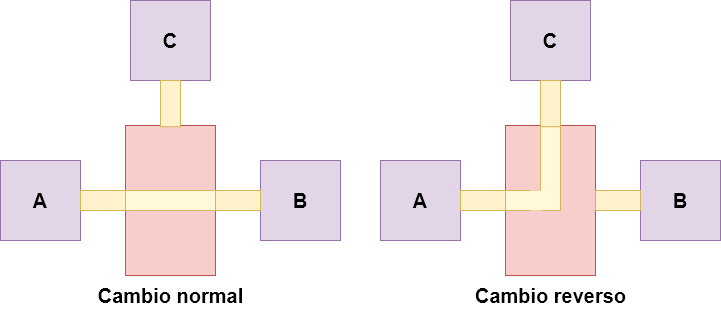
\includegraphics[scale=.5]{./Figures/FSMD-Conexiones}
		\caption{Conexión del módulo de la máquina de cambios}
		\label{fig:Cambio_conexion}
	\end{figure}	
	
	De esta manera, el nodo A ejemplificado en la Figura \ref{fig:Cambio_conexion} tendrá como vecino posterior al que le indique la máquina de cambios. Si la posición del cambio es normal, entonces el nodo A tendrá como vecino posterior al nodo B. Si la posición del cambio es reversa, entonces el nodo A tendrá como vecino posterior al nodo C.
	
	De la misma manera los nodos B y C verán como nodo "anterior" al nodo A o a ningún nodo, según el cambio se encuentre en posición normal o reversa respectivamente.	
	
	En la Figura \ref{fig:FSMD_Cambio} se ilustra el diagrama en bloques del módulo de la máquina de cambios.
	
	\begin{figure}[h]
	\centering
	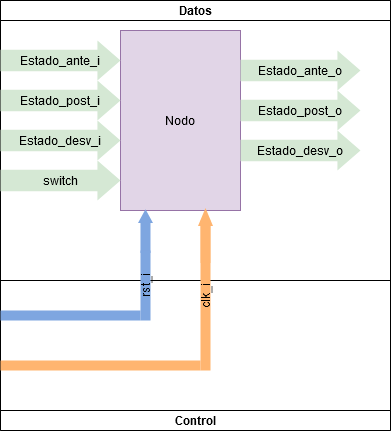
\includegraphics[scale=.5]{./Figures/FSMD-Cambio}
		\caption{FSMD del módulo de máquina de cambios}
		\label{fig:FSMD_Cambio}
	\end{figure}
		
	
\section{Módulos de adaptación a enclavamiento}

	El módulo de enclavamientos espera como entradas un vector de elementos booleanos de tamaño N y su salida será el mismo vector pero reducido a un tamaño M. Es por eso que es necesario el introducir dos módulos de adaptación. El primero debe separar el vector de N elementos booleanos (Tabla \ref{Trama_in}) en las señales que el enclavamiento necesita y el segundo debe recibir las señales de salida del sistema de enclavamiento (Tabla \ref{Trama_out}) y volver a generar el vector de elementos booleanos, que al no tener el estado de ocupación ahora tendrá un tamaño M menor que el N original. 
	 
	\begin{table}[!hbt]
	\renewcommand{\arraystretch}{1.3}
	\caption{Trama de datos a recibir}
	\label{Trama_in}
	\centering
	\begin{tabular}{| c | c | c | c |}
	\multicolumn{4}{c}{Trama de entrada [N]} \\
	\hline
	Ocupacion & Semaforos & Barreras & Cambios \\	
	\hline
	\end{tabular}
	\end{table}	 
	
	\begin{table}[!hbt]
	\renewcommand{\arraystretch}{1.3}
	\caption{Trama de datos a enviar}
	\label{Trama_out}
	\centering
	\begin{tabular}{| c | c | c | c |}
	\multicolumn{4}{c}{Trama de salida [M]} \\
	\hline
	 & Semaforos & Barreras & Cambios \\
	\hline	
	\end{tabular}
	\end{table}	
	 
	La información de la ocupación tendrá tantos elementos como circuitos de vía a modelar, donde cada tramo libre se modelará con un 1 y cada ocupado con un 0. De igual forma para barreras y cambios.
	
	La única diferencia es en el caso de los semáforos donde la información de cada semáforo no ocupará un bit sino dos bits, de forma tal de tener cuatro posibles aspectos: rojo (00), amarillo (01), doble amarillo (10) y verde (11).
	 
	\subsection{Módulo separador}
	
		En la Figura \ref{fig:FSMD_Separador} se puede ver la FSMD del módulo separador. El mismo debe recibir el vector de elementos booleanos de tamaño N (paquete[N]) y la orden de que debe procesarlo(procesar). 
		\begin{figure}[h]
		\centering
			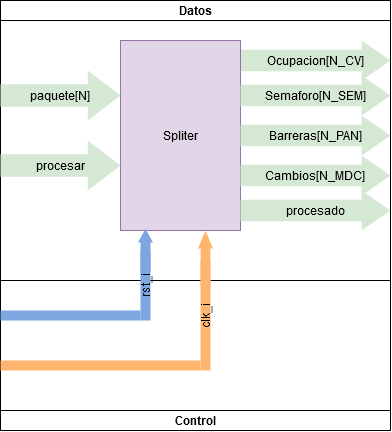
\includegraphics[scale=.5]{./Figures/FSMD-Separador}
			\caption{FSMD del módulo separador}
			\label{fig:FSMD_Separador}
		\end{figure}
		
		A continuación, como el generador de código sabe previamente la cantidad de cada uno de los elementos ferroviarios separa el paquete, puede descomponer de forma sencilla los elementos del vector paquete[N] en verctores (o variables) mas pequeñas según corresponda.
		
	\subsection{Módulo mediador}
	
		El bloque mediador que se puede visualizar en la Figura \ref{fig:FSMD_Mediador} tiene como función volver a generar el vector de elementos booleanos que ya han sido procesados por el enclavamiento.
		
		\begin{figure}[h]
		\centering
			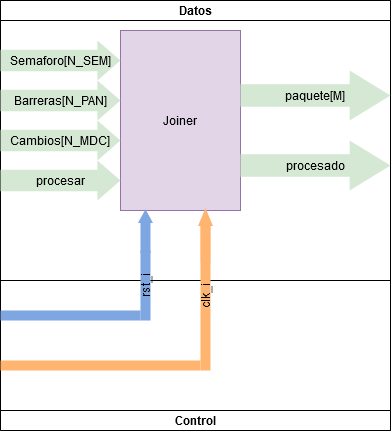
\includegraphics[scale=.5]{./Figures/FSMD-Mediador}
			\caption{FSMD del módulo mediador}
			\label{fig:FSMD_Mediador}
		\end{figure}
		
		Recibe la salida del enclavamiento y la orden de generar el paquete (procesar). Una vez que el vector (paquete[M]) ha sido creado se envía una variable de control (procesado) a la siguiente etapa para poder coordinar todo el sistema con un solo reloj.
		


\section{Módulos de procesamiento de tramas}

	Durante el desarrollo del trabajo de la Especialización en Sistemas Embebidos se había considerado la estrategia de obtener las señales de forma paralela, es decir, para cada elemento se tenía asignado un pin que monitoreaba su estado. Esto resulto ser un problema a la hora de implementar topologías mas grandes, necesitando hasta 5 veces la cantidad de entradas digitales que la plataforma tenía. Por lo tanto se decidió cambiar a una lectura y escritura en serie.
	
	Pero el utilizar una lectura serie implica que debe indicarse cual es el inicio y el final de cada mensaje, además de un criterio para determinar si el mensaje recibido es fiable.
	
	\subsection{Módulo detector}
	
		El módulo detector tiene como función el recibir una secuencia de caracteres y armar una salida con un vector de elementos booleanos. Un diagrama en bloques del funcionamiento del módulo se muestra en la Figura \ref{fig:FSMD_Detector}
		
		\begin{figure}[h]
		\centering
			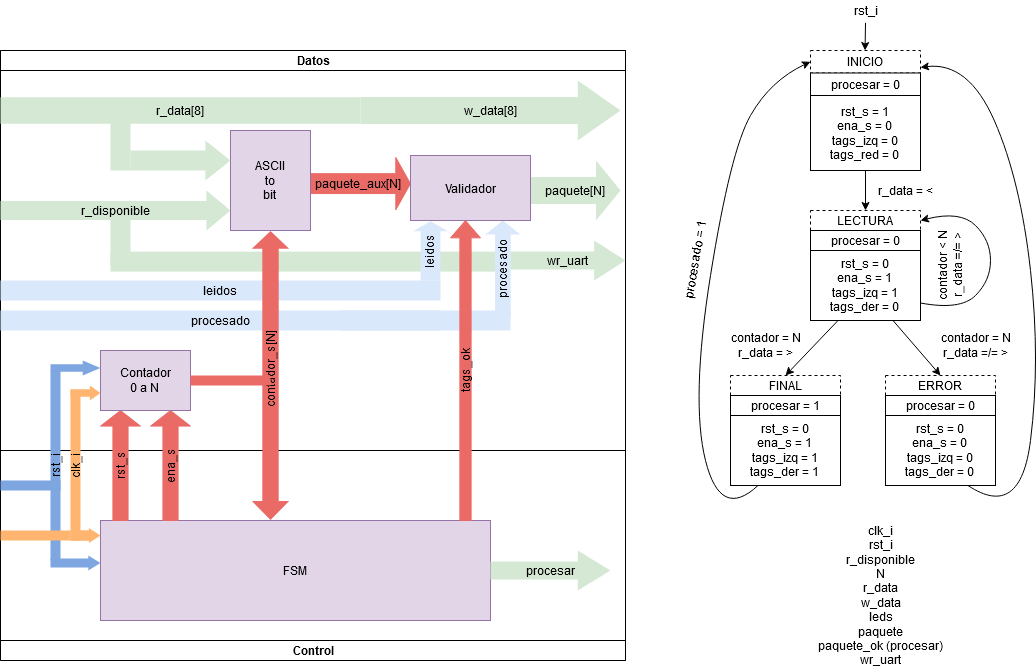
\includegraphics[scale=.6]{./Figures/FSMD-Detector}
			\caption{FSMD del módulo detector}
			\label{fig:FSMD_Detector}
		\end{figure}
		
		\vspace{5cm}
		
		La Uart envía secuencialmente un caracter por medio de la señal r\_data (8 bytes) y un pulso (r\_disponible) para informar que un nuevo dato ha sido enviado, además de indicar por medio de la señal N la cantidad de caracteres que serán enviados. 
		
		El proceso de detección es ilustrado en la Figura \ref{fig:Estados_Detector}.  		
		
		\begin{figure}[h]
		\centering
			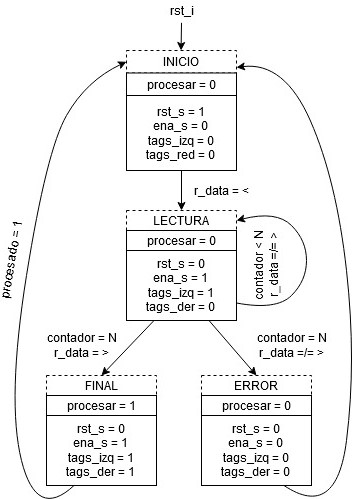
\includegraphics[scale=.65,angle = -90]{./Figures/Estados-Detector}
			\caption{Estados del módulo detector}
			\label{fig:Estados_Detector}
		\end{figure}
		
		\vspace{10cm}
		
		Se tiene un estado inicial en el cual se espera el caracter de inicio de la trama ("$<$") que provoca una transición al estado de lectura. En dicho estado se recibirán hasta N caracteres mientras se actualiza un contador interno. Cuando el contador interno iguale la cantidad N se verifica si el próximo caracter es el de fin de trama ("$>$").
		
		Si el caracter leído es el de final de trama se pasa al estado final donde el paquete es considerado válido y enviado a la próxima etapa junto con su pulso de validación del dato. Si el caracter leído es distinto, entonces se descarta toda la trama y se vuelve al inicio a la espera de otro caracter de inicio de trama, reiniciando todas las variables auxiliares.
		
		Internamente se tienen varias variables auxiliares para controlar si se han recibido los delimitadores y si la cantidad recibida es correcta. Eso cobra gran importancia al realizar los ensayos porque se puede diferenciar rápidamente la fuente de posibles errores.
		
	\subsection{Módulo registro}
	
		Así como el módulo de detección realizaba una conversión de caracteres (1 byte) a booleanos (1 bit), el módulo de registro (Figura \ref{fig:FSMD_Registro}) hace la operación inversa. Dado un vector de elementos booleanos, el módulo debe generar M caracteres '0' o '1' según corresponda en base al vector y enviarlos a la Uart para su posterior impresión.
		
		\begin{figure}[h]
		\centering
			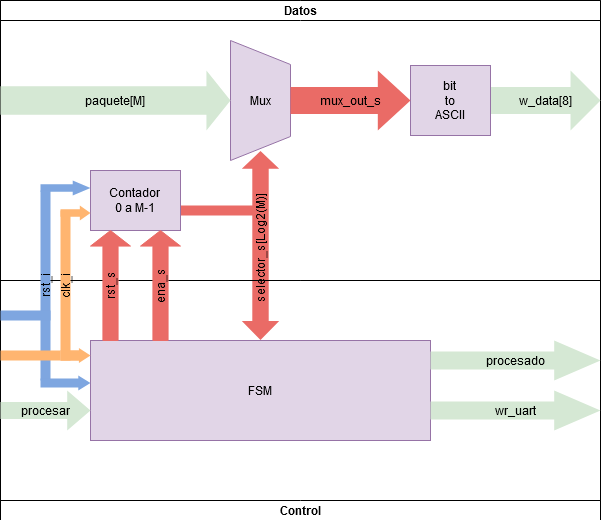
\includegraphics[scale=.6]{./Figures/FSMD-Registro}
			\caption{FSMD del módulo registro}
			\label{fig:FSMD_Registro}
		\end{figure}

		\vspace{10cm}
		
		La máquina de estados (FSM) se ocupa de generar cada dos ciclos de reloj un pulso para poder enviar secuencialmente los caracteres detectados. A la vez que el multiplexor va seleccionando cada elemento del vector paquete[M] según el valor del contador vigente, que se incrementa cada pulso del reloj interno generado.
		
		Finalmente se envía un caracter ASCII "1" si el elemento i-ésimo del paquete es '1' lógico y un "0" si lo recibido es un '0' lógico. Junto con el caracter se envía la señal wr\_uart para indicarle a la Uart que ese dato debe ser guardado en la FIFO de salida y la señal procesado para indicarle al módulo de detección que ya puede recibir nuevas tramas.
	
		La máquina de estados es ilustrada en la Figura \ref{fig:Estado_Registro}. Se añadieron dos estados para generar el pulso de reloj necesario para mantener sincronizadas las tramas y el estado de reinicio se accede al sobrepasar el tamaño máximo del contador interno que es igual a M, la cantidad de elementos esperados.
		
		\begin{figure}[h]
		\centering
			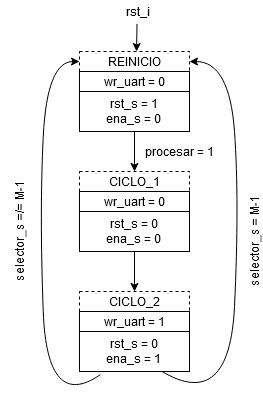
\includegraphics[scale=.9, angle = -90]{./Figures/Estados-Registro}
			\caption{Estados del módulo registro}
			\label{fig:Estado_Registro}
		\end{figure}
		
		%\vspace{10cm}
		
		La señal procesar es recibida de las etapas anteriores, si la trama ingresada es incorrecta o si ya fue impresa entonces esa señal será '0' y el registro deja de enviar datos a la UART. En caso afirmativo (procesar = '1') el proceso continuará hasta que la UART indique que no pueda recibir mas datos o que alguna etapa previa informe de algún error en el proceso.
		
	\subsection{Módulo selector}
	
		Para facilitar el proceso de desarrollo se añadió la posibilidad de elegir con uno de los switchs del kit de desarrollo el puntear completamente el enclavamiento. Es decir, con una posición del switch la salida era una copia exacta de la entrada, permitiendo diseñar todo el proceso de detección, lectura y escritura en la UART de forma independiente al enclavamiento. Mientras que con la otra posición del switch se enviaba la señal de entrada el sistema de enclavamiento y la salida era la consecuencia de haber pasado por este proceso.
		
		En la Figura \ref{fig:FSMD_Selector} se ilustra brevemente este módulo.
		
		\begin{figure}[h]
		\centering
			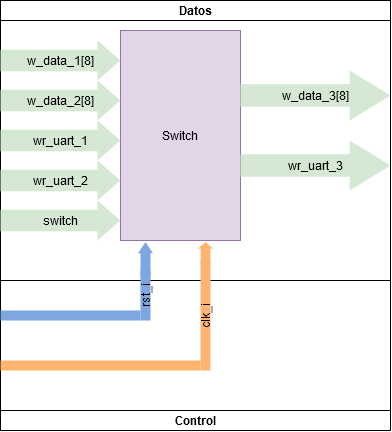
\includegraphics[scale=.6]{./Figures/FSMD-Selector}
			\caption{Diagrama de estados finitos digitales del módulo selector}
			\label{fig:FSMD_Selector}
		\end{figure}	
		
		\vspace{5cm}
		
		La implementación es por demás sencilla: un selector que decide enviar la entrada a una salida u otra según la posición del switch, de forma asincrónica. Aunque no solo envía el dato sino también la ráfaga de pulsos asociada para su correcta escritura en la UART.
		
\section{Módulo de comunicación UART}

	Para el diseño de los módulos para la interface UART con el exterior se utilizó un modelo básico aportado por los docentes, pero fueron necesarias varias premisas para modificarlo y poder automatizarlo:
	
	\begin{itemize}
		\item Se deben tener dos FIFOS distintas, una de entrada y la otra de salida.
		\item El tamaño de las FIFOs debe adaptarse a la topología: redes mas grandes necesitarán FIFOs mas grandes y redes mas pequeñas requerirán FIFOs mas pequeñas.
		\item Ambas FIFOS no pueden tener tamaño idéntico.
		\item Se deben incluir señales que indiquen al sistema si se tienen nuevos datos del exterior o si es posible recibir nuevos datos procesados para su posterior impresión.
		\item Cada cierto tiempo ambas FIFOS deberán vaciarse en su totalidad.		
	\end{itemize}
	
		Se presenta en la Figura \ref{fig:FSMD_UART} un diagrama en bloques de la UART.
			
		\begin{figure}[h]
		\centering
		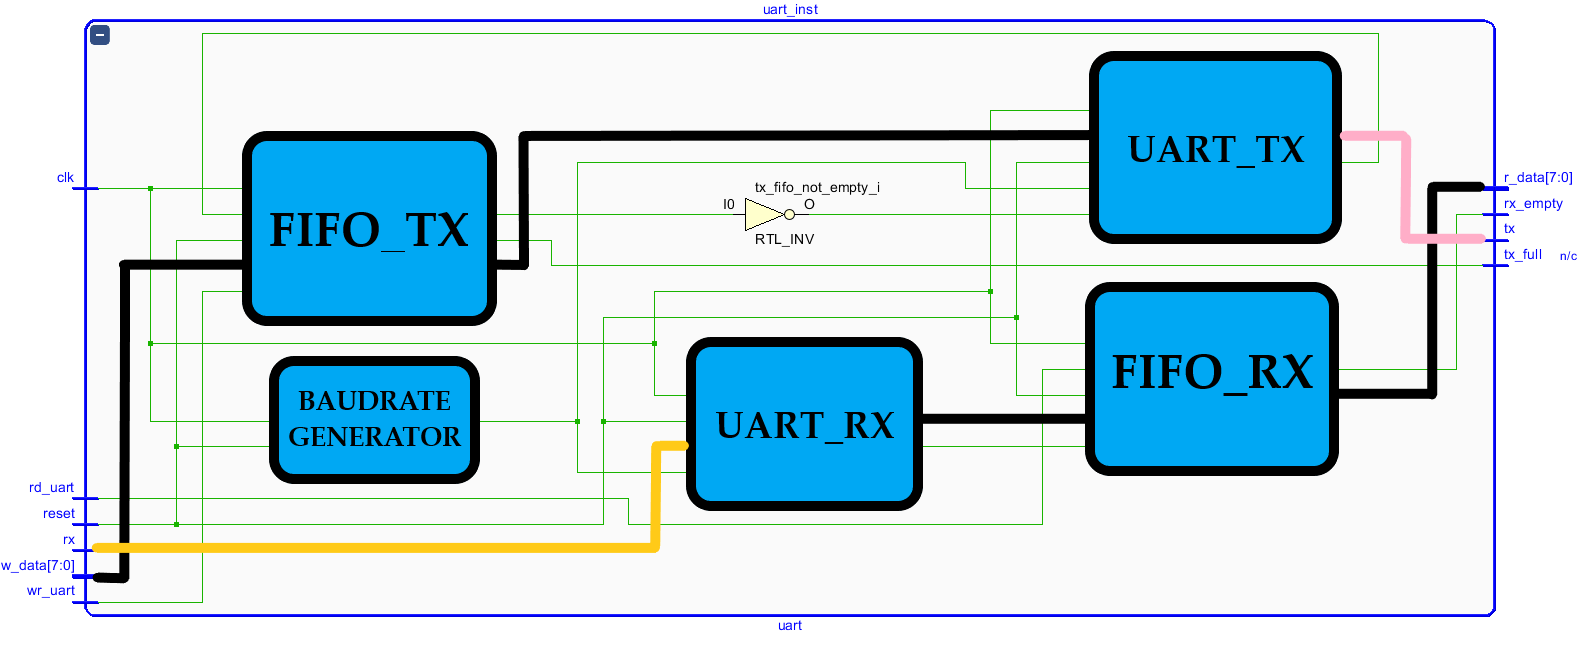
\includegraphics[scale=.35]{./Figures/UART}
			\caption{Diagrama en bloques de la UART}
			\label{fig:FSMD_UART}
		\end{figure}

		Los bloques de las FIFOs internamente son el mismo bloque, pero son instanciados de forma diferente para que adopten tamaños distintos y sean conectados a señales distintas, ya que su rol no es el mismo. La FIFO de entrada es la encargada de almacenar los valores ingresados en la plataforma con un baud-rate definido y envía su contenido al sistema junto con una serie de pulsos para indicar cuando deben ser leídos. La FIFO de salida, en cambio, debe almacenar los resultados del sistema según una serie de pulsos generada por el mismo sistema. Para luego imprimir el resultado por el puerto serie con el baud-rate definido.

		La FIFO de entrada se utiliza para almacenar una trama de la forma "<Mensaje de largo N>" por lo que espera al menos N+2 bytes, mientras que la FIFO de salida espera mensajes de la forma "Mensaje de largo M" que mide M bytes. Ya que N > M es claro que N + 2 > M en la mayoría de los casos. Aunque también puede ocurrir que la diferencia entre ambos no sea tanta y al implementar el tamaño de las FIFOs en potencias de 2 terminen ambas FIFOs con el mismo tamaño. 

		Con este criterio de diseño, en todos los demás casos, la FIFO de salida deberá ser $50\%$ menor que la de entrada, representando un ahorro de $25\%$ de los recursos estimados.
		
\section{Interfaz de comunicación Python}

	El algoritmo analizador de redes finaliza ejecutando la conexión de la consola utilizada con la plataforma FPGA. Presentando al usuario un menú de opciones para ocupar/desocupar ciertos tramos de la vía, cambiar el aspecto de ciertos semáforos, pedir que una barrera suba o baje o incluso el modificar la posición de una máquina de cambios.
	
	En la Figura \ref{fig:Menu_UART} se ilustra el menú diseñado para ingresar los comandos al sistema. Ya que existe una interfaz mucho mas avanzada desarrollada por otra parte del equipo de investigación en UTN Haedo, no se ha invertido demasiado tiempo en tener una interfaz propia para realizar pruebas a mayor escala.
	
		\begin{figure}[h]
		\centering
		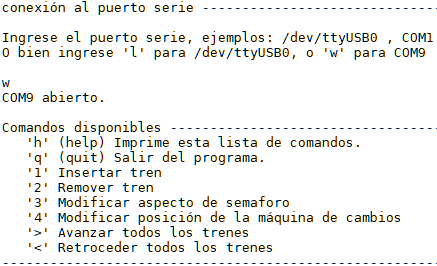
\includegraphics[scale=.76]{./Figures/Test/UART_2}
			\caption{Menú de opciones para comunicarse con el sistema}
			\label{fig:Menu_UART}
		\end{figure}
	
	\vspace{5cm}
	
	Todos los cambios repercuten en el grafo mostrado en pantalla que cambiará los colores de los semáforos y los colores de los nodos para representar la ocupación del tren. Así como también el color de las aristas para indicar la posición de los cambios.
